\documentclass[10pt,journal]{IEEEtran}
%\documentclass[conference]{IEEEtran}
%\usepackage[margin=1.5in]{geometry}
%\documentclass[11pt,a4paper]{report}
% *** GRAPHICS RELATED PACKAGES ***
%
%\ifCLASSINFOpdf
  % \usepackage[pdftex]{graphicx}
  % declare the path(s) where your graphic files are
  % \graphicspath{{../pdf/}{../jpeg/}}
  % and their extensions so you won't have to specify these with
  % every instance of \includegraphics
  % \DeclareGraphicsExtensions{.pdf,.jpeg,.png}
%\else
  % or other class option (dvipsone, dvipdf, if not using dvips). graphicx
  % will default to the driver specified in the system graphics.cfg if no
  % driver is specified.
  % \usepackage[dvips]{graphicx}
  % declare the path(s) where your graphic files are
  % \graphicspath{{../eps/}}
  % and their extensions so you won't have to specify these with
  % every instance of \includegraphics
  % \DeclareGraphicsExtensions{.eps}
%\fi
% graphicx was written by David Carlisle and Sebastian Rahtz. It is
% required if you want graphics, photos, etc. graphicx.sty is already
% installed on most LaTeX systems. The latest version and documentation can
% be obtained at:
% http://www.ctan.org/tex-archive/macros/latex/required/graphics/
% Another good source of documentation is "Using Imported Graphics in
% LaTeX2e" by Keith Reckdahl which can be found as epslatex.ps or
% epslatex.pdf at: http://www.ctan.org/tex-archive/info/
%
% latex, and pdflatex in dvi mode, support graphics in encapsulated
% postscript (.eps) format. pdflatex in pdf mode supports graphics
% in .pdf, .jpeg, .png and .mps (metapost) formats. Users should ensure
% that all non-photo figures use a vector format (.eps, .pdf, .mps) and
% not a bitmapped formats (.jpeg, .png). IEEE frowns on bitmapped formats
% which can result in "jaggedy"/blurry rendering of lines and letters as
% well as large increases in file sizes.
%
% You can find documentation about the pdfTeX application at:
% http://www.tug.org/applications/pdftex





% *** MATH PACKAGES ***
%
\usepackage[cmex10]{amsmath}
% A popular package from the American Mathematical Society that provides
% many useful and powerful commands for dealing with mathematics. If using
% it, be sure to load this package with the cmex10 option to ensure that
% only type 1 fonts will utilized at all point sizes. Without this option,
% it is possible that some math symbols, particularly those within
% footnotes, will be rendered in bitmap form which will result in a
% document that can not be IEEE Xplore compliant!
%
% Also, note that the amsmath package sets \interdisplaylinepenalty to 10000
% thus preventing page breaks from occurring within multiline equations. Use:
%\interdisplaylinepenalty=2500
% after loading amsmath to restore such page breaks as IEEEtran.cls normally
% does. amsmath.sty is already installed on most LaTeX systems. The latest
% version and documentation can be obtained at:
% http://www.ctan.org/tex-archive/macros/latex/required/amslatex/math/





% *** SPECIALIZED LIST PACKAGES ***
%
%\usepackage{algorithmic}
% algorithmic.sty was written by Peter Williams and Rogerio Brito.
% This package provides an algorithmic environment fo describing algorithms.
% You can use the algorithmic environment in-text or within a figure
% environment to provide for a floating algorithm. Do NOT use the algorithm
% floating environment provided by algorithm.sty (by the same authors) or
% algorithm2e.sty (by Christophe Fiorio) as IEEE does not use dedicated
% algorithm float types and packages that provide these will not provide
% correct IEEE style captions. The latest version and documentation of
% algorithmic.sty can be obtained at:
% http://www.ctan.org/tex-archive/macros/latex/contrib/algorithms/
% There is also a support site at:
% http://algorithms.berlios.de/index.html
% Also of interest may be the (relatively newer and more customizable)
% algorithmicx.sty package by Szasz Janos:
% http://www.ctan.org/tex-archive/macros/latex/contrib/algorithmicx/




% *** ALIGNMENT PACKAGES ***
%
%\usepackage{array}
% Frank Mittelbach's and David Carlisle's array.sty patches and improves
% the standard LaTeX2e array and tabular environments to provide better
% appearance and additional user controls. As the default LaTeX2e table
% generation code is lacking to the point of almost being broken with
% respect to the quality of the end results, all users are strongly
% advised to use an enhanced (at the very least that provided by array.sty)
% set of table tools. array.sty is already installed on most systems. The
% latest version and documentation can be obtained at:
% http://www.ctan.org/tex-archive/macros/latex/required/tools/

\usepackage{multirow}
\usepackage{mdwmath}
\usepackage{mdwtab}
% Also highly recommended is Mark Wooding's extremely powerful MDW tools,
% especially mdwmath.sty and mdwtab.sty which are used to format equations
% and tables, respectively. The MDWtools set is already installed on most
% LaTeX systems. The lastest version and documentation is available at:
% http://www.ctan.org/tex-archive/macros/latex/contrib/mdwtools/


% IEEEtran contains the IEEEeqnarray family of commands that can be used to
% generate multiline equations as well as matrices, tables, etc., of high
% quality.


%\usepackage{eqparbox}
% Also of notable interest is Scott Pakin's eqparbox package for creating
% (automatically sized) equal width boxes - aka "natural width parboxes".
% Available at:
% http://www.ctan.org/tex-archive/macros/latex/contrib/eqparbox/





% *** SUBFIGURE PACKAGES ***
%\usepackage[tight,footnotesize]{subfigure}
% subfigure.sty was written by Steven Douglas Cochran. This package makes it
% easy to put subfigures in your figures. e.g., "Figure 1a and 1b". For IEEE
% work, it is a good idea to load it with the tight package option to reduce
% the amount of white space around the subfigures. subfigure.sty is already
% installed on most LaTeX systems. The latest version and documentation can
% be obtained at:
% http://www.ctan.org/tex-archive/obsolete/macros/latex/contrib/subfigure/
% subfigure.sty has been superceeded by subfig.sty.



\usepackage[caption=true]{caption}
%\usepackage[font=footnotesize]{subfig}
% subfig.sty, also written by Steven Douglas Cochran, is the modern
% replacement for subfigure.sty. However, subfig.sty requires and
% automatically loads Axel Sommerfeldt's caption.sty which will override
% IEEEtran.cls handling of captions and this will result in nonIEEE style
% figure/table captions. To prevent this problem, be sure and preload
% caption.sty with its "caption=false" package option. This is will preserve
% IEEEtran.cls handing of captions. Version 1.3 (2005/06/28) and later
% (recommended due to many improvements over 1.2) of subfig.sty supports
% the caption=false option directly:
%\usepackage[caption=false,font=footnotesize]{subfig}
%
% The latest version and documentation can be obtained at:
% http://www.ctan.org/tex-archive/macros/latex/contrib/subfig/
% The latest version and documentation of caption.sty can be obtained at:
% http://www.ctan.org/tex-archive/macros/latex/contrib/caption/




% *** FLOAT PACKAGES ***
%
%\usepackage{fixltx2e}
% fixltx2e, the successor to the earlier fix2col.sty, was written by
% Frank Mittelbach and David Carlisle. This package corrects a few problems
% in the LaTeX2e kernel, the most notable of which is that in current
% LaTeX2e releases, the ordering of single and double column floats is not
% guaranteed to be preserved. Thus, an unpatched LaTeX2e can allow a
% single column figure to be placed prior to an earlier double column
% figure. The latest version and documentation can be found at:
% http://www.ctan.org/tex-archive/macros/latex/base/



\usepackage{stfloats}
% stfloats.sty was written by Sigitas Tolusis. This package gives LaTeX2e
% the ability to do double column floats at the bottom of the page as well
% as the top. (e.g., "\begin{figure*}[!b]" is not normally possible in
% LaTeX2e). It also provides a command:
%\fnbelowfloat
% to enable the placement of footnotes below bottom floats (the standard
% LaTeX2e kernel puts them above bottom floats). This is an invasive package
% which rewrites many portions of the LaTeX2e float routines. It may not work
% with other packages that modify the LaTeX2e float routines. The latest
% version and documentation can be obtained at:
% http://www.ctan.org/tex-archive/macros/latex/contrib/sttools/
% Documentation is contained in the stfloats.sty comments as well as in the
% presfull.pdf file. Do not use the stfloats baselinefloat ability as IEEE
% does not allow \baselineskip to stretch. Authors submitting work to the
% IEEE should note that IEEE rarely uses double column equations and
% that authors should try to avoid such use. Do not be tempted to use the
% cuted.sty or midfloat.sty packages (also by Sigitas Tolusis) as IEEE does
% not format its papers in such ways.





% *** PDF, URL AND HYPERLINK PACKAGES ***
%
%\usepackage{url}
% url.sty was written by Donald Arseneau. It provides better support for
% handling and breaking URLs. url.sty is already installed on most LaTeX
% systems. The latest version can be obtained at:
% http://www.ctan.org/tex-archive/macros/latex/contrib/misc/
% Read the url.sty source comments for usage information. Basically,
% \url{my_url_here}.





% *** Do not adjust lengths that control margins, column widths, etc. ***
% *** Do not use packages that alter fonts (such as pslatex).         ***
% There should be no need to do such things with IEEEtran.cls V1.6 and later.
% (Unless specifically asked to do so by the journal or conference you plan
% to submit to, of course. )
\usepackage[T1]{fontenc}% optional T1 font encoding
\usepackage[pdftex]{graphicx}
\usepackage{float}
%\usepackage{lipsum}
\usepackage{placeins}
\usepackage{array}
\usepackage{pdflscape}
\usepackage{afterpage}
\usepackage{rotating}
\usepackage{epstopdf}
\usepackage{bbding}
\usepackage{pifont}
\usepackage{ctable}
%\newcommand{\cmark}{\ding{51}}%
\newcommand{\xmark}{\ding{55}}%
\usepackage{wasysym}
%\usepackage{enumitem}
\usepackage{amssymb}
\usepackage{graphicx}
\usepackage{caption}
\usepackage{subcaption}
%\usepackage{algorithm2e}
%\usepackage{algorithm,algorithmic}
%\usepackage{algpseudocode}
%\usepackage{algorithm}
%\usepackage[noend]{algpseudocode}
\usepackage [linesnumbered, ruled, vlined] {algorithm2e}
%\usepackage[options ]{algorithm2e}
\usepackage{authblk}
%\usepackage[T1]{fontenc}
%\usepackage{tikz}
%\usetikzlibrary{arrows,calc,postioning}
\newcolumntype{L}[1]{>{\raggedright\let\newline\\\arraybackslash\hspace{0pt}}m{#1}}
\newcolumntype{C}[1]{>{\centering\let\newline\\\arraybackslash\hspace{0pt}}m{#1}}
\newcolumntype{R}[1]{>{\raggedleft\let\newline\\\arraybackslash\hspace{0pt}}m{#1}}
% correct bad hyphenation here
\hyphenation{op-tical net-works semi-conduc-tor}
%\usepackage{csquotes}
\usepackage{textcomp}
 
\begin{document}



\title{An Improved Prophet - Machine Learning Based Optimized Multi-Copy Routing Algorithm for IoT and Opportunistic Mobile Networks}


%
% paper title
% can use linebreaks \\ within to get better formatting as desired
\title{An Improved Prophet - Machine Learning Based Optimized Multi-Copy Routing Algorithm for IoT and Opportunistic Mobile Networks}
\author[$\dag$ ]{Srinidhi N N, Sagar C S, Deepak Chethan S, Vinay G P, Vaishak, Dilip Kumar S M} 
\affil[$\dag$]{\emph{Dept. of Computer Science and Engineering, University Visvesvaraya College of Engineering, Bangalore, India}}

\affil[.]{\emph{srinidhinagesh@gmail.com}}
%\affil[$\ddagger$]{\emph{raghush86@gmail.com}}
%\affil[$\mathsection$]{\emph{zhengzhigao@hust.edu.cn}}
%\affil[$\|$]{\emph{Mohamed_elhoseny@mans.edu.eg}}


%\author{Vinay~K,~\IEEEmembership{Student~Member,~IEEE,}
%        Dilip~Kumar~S~M,~\IEEEmembership{Member,~IEEE,}
%        and~Venugopal~K~R,~\IEEEmembership{Fellow,~IEEE}% <-this % stops a space
%\thanks{Vinay K was with the Department
%of Computer Science and Engineering, University Visvesvaraya College of Engineering, Bengaluru,
%India e-mail:ec.vinay@gmail.com.}% <-this % stops a space
%\thanks{Dilip Kumar S M and Venugopal K R are with University Visvesvaraya College of Engineering, Bengaluru,
%India.}% <-this % stops a space
%\thanks{Manuscript received April 19, 2005; revised August 26, 2015.}}
%
%}
%\and
%\IEEEauthorblockN{Dilip Kumar S M}
%\IEEEauthorblockA{Dept of Computer Science and Engineering\\UVCE, Bangalore\\
%Email: dilipkumarsm@gmail.com}}
% conference papers do not typically use \thanks and this command
% is locked out in conference mode. If really needed, such as for
% the acknowledgment of grants, issue a \IEEEoverridecommandlockouts
% after \documentclass
% for over three affiliations, or if they all won't fit within the width
% of the page, use this alternative format:
%\author{\IEEEauthorblockN{Michael Shell\IEEEauthorrefmark{1},
%Homer Simpson\IEEEauthorrefmark{2},
%James Kirk\IEEEauthorrefmark{3},
%Montgomery Scott\IEEEauthorrefmark{3} and
%Eldon Tyrell\IEEEauthorrefmark{4}}
%\IEEEauthorblockA{\IEEEauthorrefmark{1}School of Electrical and Computer Engineering\\
%Georgia Institute of Technology,
%Atlanta, Georgia 30332--0250\\ Email: see http://www.michaelshell.org/contact.html}
%\IEEEauthorblockA{\IEEEauthorrefmark{2}Twentieth Century Fox, Springfield, USA\\
%Email: homer@thesimpsons.com}
%\IEEEauthorblockA{\IEEEauthorrefmark{3}Starfleet Academy, San Francisco, California 96678-2391\\
%Telephone: (800) 555--1212, Fax: (888) 555--1212}
%\IEEEauthorblockA{\IEEEauthorrefmark{4}Tyrell Inc., 123 Replicant Street, Los Angeles, California 90210--4321}}
% use for special paper notices
%\IEEEspecialpapernotice{(Invited Paper)}
% make the title area
\maketitle
\begin{abstract}

Opportunistic networks are one of the important categories of adhoc networks in Internet of Things (IoT), which exploits human social characteristics like daily routines, similarities etc., to facilitate sending and receiving of messages. In Opportunistic networks, mobile nodes are used to establish communication between nodes despite of non-availability of a dedicated route between them. Furthermore, nodes don\textquotesingle t acquire any knowledge in advance about the characteristics of the network such as the network topology, the location of the other nodes. Hence, designing a routing algorithm becomes a challenging task since traditional routing protocols used in the Internet are not feasible for the characteristics inherent in this type of network. The proposed work propounds a multi-copy routing algorithm based on machine learning named iProphet or improved Prophet. iProphet, uses dynamically changing contextual information of nodes and the delivery probability of Prophet to carry out message transfer. The multi-copy routing algorithm uses a machine learning classifier known as random forest to classify the node as a good forwarder or a bad forwarder based on the supplied contextual information during each routing decision. The classifier trained with large amount of data extracted using simulation leads to precise classification of the nodes as reliable or unreliable for carrying out the routing task. The simulation results show that the proposed algorithm outperforms with respect to delivery probability, hop count, overhead ratio, latency but over costs with respect to average buffer time in par with similar multi-copy routing algorithm. The uniqueness of this paper lies in data extraction, categorization and training the model to obtain reliable and unreliable nodes to provide efficient multi-copy routing in IoT scenario.    

\end{abstract}
\vspace{0.5cm} 
\begin{IEEEkeywords}
Internet of Things, Machine Learning, Mobility, Multi-Copy, Random Forest
\end{IEEEkeywords}
%\textbf{\textit{Index Terms}-Cloud Computing, Scientific Workflows, SWfMS.}
%----------------------------------------------------------------------------------------------------------------------------------
% IEEEtran.cls defaults to using nonbold math in the Abstract.
% This preserves the distinction between vectors and scalars. However,
% if the conference you are submitting to favors bold math in the abstract,
% then you can use LaTeX's standard command \boldmath at the very start
% of the abstract to achieve this. Many IEEE journals/conferences frown on
% math in the abstract anyway.

% no keywords




% For peer review papers, you can put extra information on the cover
% page as needed:
% \ifCLASSOPTIONpeerreview
% \begin{center} \bfseries EDICS Category: 3-BBND \end{center}
% \fi
%
% For peerreview papers, this IEEEtran command inserts a page break and
% creates the second title. It will be ignored for other modes.
%\IEEEpeerreviewmaketitle
%\vspace{-0.7cm}
\section{Introduction}
With the development in technogies, more and more devices are getting connected to the Internet, which is heading to the new criterion in computing and communication known as the Internet of Things (IoT) \cite{iot2010}. As a result, more devices are getting prevalently monitored and cannot be deployed statically. These IoT devices while being transported by humans or different carriers will interact either statically or dynamically. For instance, in vehicular based IoT network statically deployed devices may necessitate to recognize the mobile agents and employ them in assembling and delivering their information to the intended target \cite{srinidhi2018network}. 
Along the way opportunistic mobile networks \cite{2006opnet} rose as a novel mechanism of transmissions in wireless systems. Unlike mobile ad hoc networks (MANETs) that needs end-to-end connection routes for information transfer, the communication in opportunistic mobile networks takes place on the corporation of opportunistic connections among mobile nodes, without the availability of end-to-end communication paths. These mobile devices establishes connection when people comes in contact and these network type are considered as human social networks. Hence, the opportunistic networks utilize the individual behaviors and social relations to provide more effective and reliable message distribution systems. In OppIoT \cite{iot2013}, data acquisition, propagation, and distribution of data which typically necessitate opportunistic connections utilizing mobility, short-range transmission, and technologies. During such operations, the configuration of the routing protocol is a challenging task due to this inherent complexity in securing connectivity among devices and recognizing a relevant data packet forwarder that can convey the packet to its desired destination.
These networks  are the derived class of OppIoT and considered as evolved form of MANETs. In OppNets, nodes are allowed to communicate with several other nodes even though a routing connecting does not exist between them. Nodes are connected momentarily and the routes keep dynamically changing due to nodes mobility or  frequent nodes activation and deactivation. When the packets are en route between the source node and the target node(s), any viable node can be opportunistically employed as the next hop, granted it is plausible to bring the packet closer to the intended destination. 
Several protocols related to OppNets that have been proposed such as epidemic, HBPR, HibOp etc., which uses parameters like message propagation pattern, context erudition of nodes (i.e., current position, the possibility of delivery, target node distance, prior and existing history of the node), last synergy  time and various other parameters in order to predict which node is opted  as next hop to deliver the message to the intended destination. In this work, a  machine learning based algorithm which can be employed to OppNets is proposed. The proposed algorithm that differ radically from the existing algorithm as this algorithm uses  the random forest to decide the neighboring node to route the data packet based on the present context and location information. Random forest or otherwise referred to as random decision forest are one of the most popular ensemble learning techniques that are used in both classification and regression. Several decision trees are randomly created with several subsets of data during the training period. The class is assigned based on the mode. Random forest algorithm uses the technique of bootstrap aggregation, which helps in improving the stability and accuracy of the algorithm along with reducing the variance and overfitting of the proposed iProphet. \\
The rest of the paper is organized as follows. Section II presents a summary of various existing works with
respect to multi-copy and oppurtunisitic networks. Problem statement is presented in Section III. Proposed algorithm has been presented in section IV. The experimental evaluation and results has been explained in section V. Conclusion along with future work has been presented in Section VI. 

\section{Related Work}
Many protocols that are used in OppNets are related to the nodes context-information and message distribution. Representative ones are summed as follows.
Epidemic routing \cite{2000epi}, is a flood-based routing algorithm whose foremost objective is to deliver the packet with high probability to the desired destination with a minimum premise about the topology and the network. The work is based on epidemic algorithm which manages two buffers one for the message originating from the node itself and the other buffer is used to store messages generated from different nodes. Each node contains a summary vector that carries a short description of messages currently cached in the buffer. When nodes come in contact of one another, they revise their summary vectors and each node has an extra buffer to prevent verbose connection with other nodes. Nodes exchange their summary vector with each other after a predefined time and after exchanging their vectors the nodes rival their vectors to ascertain which message is missing. Then, the nodes request for the copies of the messages which they do not contain. But the proposed epidemic protocol uses higher bandwidth and buffer space which will cause network congestion and it do not examine nodes parameters to predict the possibility of message delivery.
The HBPR (History Based Prediction for Routing), protocol which was proposed by Dhurandher et al. \cite{2004hbpr}, uses election of the intermediate node as the message carrier is decided based on specific parameters. These parameters are the duration for which a pair of nodes meet, node's history, time at which a couple of nodes meet, and the path of the mobility of the node concerning the root and the target node. The schema consists of three stages, i.e., identifying the home location, wherein the nodes movement is utilized to recognize the subsequent mode location; the message production stage, during which the intermediate node is determined, and also the home location is renewed and lastly, the Subsequent hop selection phase, where  metric is determined to help to judge on the assortment of the best succeeding forwarder of the message. This protocol has been confirmed to produce improved results than Epidemic concerning the message delivery number and Overhead ratio, but considering the individual mobility paradigm only.
Prophet routing protocol \cite{2003pric}, uses non-arbitrary movement and association patterns in practical application situation to replicate the message to different nodes in order to enhance the routeing performance. It is established on the basis that if a node has communicated with a different node or visited a region regularly, then there is a higher likelihood of revisiting the region or the node. In order to accomplish this, a delivery probability is defined for every node which associates itself with other nodes. Let assume that a node T wants to remit a packet to node U if this node T comes in association with another node  R  which has a higher delivery probability to node U compared to T  only then a  copy of the packet is copied to the node R.
The deliverability is established based on the buffer size aggregate, position, popularity and predictability of delivery. If a source node comes in association concurrently with various nodes the message is copied to the node which has the highest value of deliverability. In distance-based Prophet, routing algorithm distance is used as an added factor. Here each node containing the packet checks the distance from all the bordering nodes and picks the nodes with is closed as the packet forwarder. Thereby improving the probability of delivery and lessening the delay probability.  
Prowait routing algorithm which was proposed by Dhurandher et. al. \cite{2015pbcffon}, can be considered as an amalgamation of the Prophet and Spray and wait routing protocol. Prowait model utilities an uncomplicated forwarding schema, in which when two nodes engage, the transaction of packet takes place from the node with lower probability of delivery to the node have higher probability concerning the desired destination. They mainly weigh a couple of parameters during packet transmission  1) election of an adjacent node 2) choosing the node for the next hop. For the election of the node, the Prophet protocol is used to estimate delivery predictability and transferring of the data is done using the spray and wait routing protocol. Choosing the node for the next hop is done using the Prophet routing algorithm. Prowait routing algorithm keeps the replicate data packets so that the packet is delivered to the intended destination with minimum delay. It reduces the usage of resource wastage by depreciating the amount of flooding compared to the epidemic protocol. It, however, does not predict forwarding of the message packet in order to improve delivery delay in the network.
HiBO protocol (history-based routing protocol for OppNets) was proposed by Boldrini et. al. \cite{hibop}. which utilizes the present context statistics about the nodes to ascertain the suitable node to convey the message to the desired destination. The context statistics are collected from the simulation environment. When the node desire to transmit the message, the node utilizes the History-Table and Identity-Table to decide, whether there is a union between the context statistic of its adjacent nodes and the data associated with the message. In that case, the data packet is transmitted to the adjacent node for which the union occurred. This routing algorithm will have higher delay in deciding which is the neighboring node and requires additional effort in maintaining the tables.
EDR(encounter and distance based routing algorithm) \cite{2016edr}, protocol uses context statistics to convey the message from the source to the destination. Here the routing protocol determines dynamically contact value for every couple of nodes (i.e. the frequency at which a pair of nodes meet). Moreover, the Euclidean distance is also estimated dynamically for every couple of nodes. A  parameter called the best-forwarder is evaluated based on the values considered earlier and the packet is transmitted to those intermediate nodes only if their forwarder value is more than the threshold. As it is context related protocol, it does not function well concerning packet delivery probability and overhead ratio.
A  Markov chain prediction model proposed by Jeon and Lee \cite{2016dmcpm}, in which given nodes mobility behavior is outlined on the given nodes former mobility information state to anticipate the nodes expected movement. Using this data, mobile nodes packet delivery ratio to destination node is calculated. The proposed protocol enhances the delivery ratio and reduces the average delay compared to conventional routing protocols for OppNets. However, this protocol performs inadequately compared to other mobility models like a random waypoint.  
MLProph \cite{2016mlbp}, which is an infrastructure-less OppNet routing protocol utilizes a machine learning procedure to decide preceding network information and nodes parameters like the size of the buffer, hop-count, momentum and delivery. Based on these parameters, node likelihood as a forwarder is determined. However, it does not take into account of node's message delivery probability which is prime parameter to be considered during routing.\\
However, in the proposed model random forest algorithm is considered to decide the neighboring node to route the data packet based on the present context and location information. Several decision trees are randomly created with several subsets of data during the training period, which helps in improving the stability and accuracy of the algorithm along with reducing the variance and overfitting.

\section{Problem statement and challenges}
\subsection{Problem statement}
There are various challenges that opportunistic network in IoT faces. This is due to the dynamic nature of nodes over time depending on the application, which makes it difficult for routing the information and to identify the intermediate nodes which are used for forwarding messages to destination.
 \begin {enumerate}

\item The problem is to classify the node as a good forwarder or a bad forwarder based on the supplied contextual information during each routing decision in order to optimize delivery probability, hop count, overhead ratio, latency.

\item To train the random forest classifier with large amount of data extracted using simulation to precise the classification of the nodes as reliable or unreliable for carrying out the routing.

\end{enumerate}

\subsection{Challenges}
\begin{itemize}
	\item Data extraction: For training the machine learning based random forest model, a huge data set had to be obtained. Trying to get data that is close to the real world was a challenge. ONE simulator provided the closest solution. To extract the data from the ONE simulator, its source code had to be modified.
	\item Model Creation: With the data extracted from ONE simulator, a robust random forest classifier had to be constructed. For doing which, features and algorithm related parameters had to be properly chosen. 
	\item Model Integration: After the model is constructed, it had to be properly integrated with the ONE simulator to classify the nodes.
\end{itemize}

%\section{System model}



\section{Proposed Algorithm}
This section provides in detail explanation of the proposed iProphet algorithm.

\subsection{Terminology}
\begin{itemize}
\item $S$: Source node 
\item $D$: Destination node 	
\item $X$: Selected forwarder node 	
\item $G$: Set of all neighboring nodes 
\item $N_i$: Neighboring node i in the set S 
\item $M_i$: Message  
\item $n$: Current node, the node tasked with making a routing decision 
\item $M$: Set of all messages that were generated during data generation phase 
\item $M_s$: Set of messages that were delivered 
\item $M_d$: Set of messages that were dropped or aborted 
\item $E$: Set of all the events recorded during data extraction phase of Prophet 
\item $P(N_i)$: Delivery probability as calculated by Prophet for the neighbor node Ni by current node n 
\item $feature\_name(x)$: Value of the attribute \emph{feature\_name} in the record x in any set. 
\end{itemize}

Consider $N$ nodes forming an opportunistic network with a means to communicate and having sufficient energy. Every node has sufficient buffer to store the state information like the nodes movement information, current location, delivery probability, direction, distance between source and destination, past history, power status. All these attributes can be used to determine the route for the message transfer. $Prophet$ (Probability routing protocol using history of encounters and transitivity) is one of the algorithm that uses previous contact history between the nodes to calculate the delivery probability between them. This is used to deliver the packets to the destination. Even though this provides a sufficient performance, the method to select the next node could be optimized by application of machine learning models. Prophet does not completely utilize all the context information present in the nodes. With the data driven approach, we can choose the best predictors/features and use them to drive the routing decisions. 
In the proposed Machine Learning Based Optimized Multi-Copy Routing Algorithm for IoT and Opportunistic Mobile Networks, random forests algorithm is used to choose the neighboring node to route the data packet based on the present context and location information.  Random forest or otherwise referred to as random decision forests are one of the most popular ensemble learning techniques that are used for both classification and regression. Several decision trees are randomly constructed with varied subsets of data during the training period. The class is assigned based on the mode. Random forest algorithm uses the technique of bootstrap aggregation, which helps in improving the stability and accuracy of the algorithm along with reducing the variance and overfitting. Formally, consider a training set $X = x_1, ..., x_n$ along with their corresponding outputs $Y = y_1, ..., y_n$ giving dataset $D_n={(X_1,Y_1),...,(X_n,Y_n)}$. Random forest is a collection of random base regression trees $\{rn(x,\theta_m,D_n),m\ge1\}$, where $\theta_1,\theta_2,...$ are outputs of a randomizing variable $\theta$. The outputs of these random trees are aggregated to get an estimate. Thus, random forest model is given by,  
\begin{equation}
	\bar{rn}(X,D_n) =E_\theta[rn(X,\theta,D_n)]
\end{equation}
Where $E_\theta$ is the expectation with respect to $\theta$. The dataset is divided into various subspaces based on this randomizing variable theta. It is also used to find out on what basis the successive cuts are done when constructing the individual trees. During the learning period, the algorithm will choose a random subset of features, called as feature bagging. If a given feature is a strong predictor, it is used repeatedly in several different trees. To find the optimal number of trees, cross-validation techniques is applied. The main advantage of Random forest over normal decision trees is that the predictions from single tree are susceptible to noise. But the aggregation of forest will overcome from this drawback. Random forest algorithm can also be viewed as weighted neighborhood schemes.   
Here random Forests algorithm is be used to classify the neighboring nodes as good and bad forwarders based on the contextual information. Our proposed algorithm has mainly three stages: (1) Collecting routing data from one simulator (2) Building and training the model (3) Application of the model
\subsection{Collecting routing data from one simulator}
ONE simulator is one of the best simulation environment for  simulating opportunistic mobile networks. For this stage, modification of the one simulator source was done to extract the necessary information to train the algorithm. A total of 4 datasets are generated, they are.
\begin{enumerate}
	\item Event Dataset:
		This dataset is used to describe every event that took place inside the simulation environment. An event is a discrete piece of entity in a discrete-event based simulation system. In our context an event represented as activity inside the environment such as relaying of the message. The features of this dataset contains the following information in columns and rows.
		\begin{enumerate}
			\item $Key$: Used to identify the inter related records in various datasets. 
			\item $current\_node$: This is the node which contains message related to routing decision. 
			\item $destination\_node$: The node to which the message has to be delivered. 
			\item $neighbor\_nodes$: The list of all the node ids which are in range to the current node. 
			\item $message\_id$: id of the message which is to be forwarded. 
			\item $selected\_forwarder$: The node selected as the forwarder for the message in Prophet algorithm. 
			\item $predictability\_of\_the\_current\_node$: Delivery prediction for the current node as calculated by the original Prophet algorithm. 
			\item $predictability\_of\_the\_selected\_forwarder$: Delivery prediction for the selected forwarder based on which it was selected as a best forwarder.  
		\end{enumerate}
	\item Message Dataset:
		    This dataset contained rows that described the details of the message like its source, intended destination, message size, the traveled path. An important feature is it contains \emph{delivery status}, which is used to know whether the message was finally delivered to the intended destination or whether it was aborted in halfway. Based on this feature, the dataset was further categorized into three parts: 
		    \begin {enumerate}
		    	 \item Delivered: This dataset contained messages that are ultimately delivered to the final destination. 
		    	\item Aborted or dropped: Messages that are dropped during routing. 
		    	\item Relayed: Messages that are transferred to intermediate nodes.  
		    \end {enumerate}
		    The features of this dataset contains the following information as columns of the row: 
		    \begin {itemize}
		    	 \item $key$: For event dataset as described earlier. 
		    	 \item $message\_id$: A unique identifier to identify the message. 
		    	 \item $message\_size$: Size of the message in bytes. 
		    	 \item $source$: Node from which the message is generated. 
		    	 \item $destination$: Node to which intended message should be delivered.
		    	 \item $number\_of\_hops$: Number of nodes traversed in its path to destination. 
		    	\item $message\_creation\_time$: Time during which message was created in simulated seconds. 
		    	 \item $message\_deletion\_time$: Time during which the message was deleted in simulated seconds.
		    \end {itemize}
	\item Event meta-data dataset: 
	This dataset described every entity like the source node, the current node, intermediate node, selected forwarder node that were involved in every event in the event dataset. 
	\begin {enumerate}
		\item Host info: Host info of the node is the set of information about the node at that particular point of event time. This includes nodes x coordinate, y coordinate, buffer size, next time to move, free buffer space, nodes speed recorded in 9 columns. 
	\end {enumerate}
		The features of this dataset contains the following information as columns of the row for every event recorded. 
	\begin {itemize}
	 \item key - as described for the above dataset 
	 \item Host info of current node  
	 \item Host info of destination node  
	 \item Host info for all the neighbors 
	 \item Id of the selected forwarder  
	 \item message\_id 
	\end {itemize}
	
	At the end of this stage, number of datasets containing sufficient number of rows were generated to pre-process the data and to train the algorithm. 
		
\end{enumerate}

\subsection{Building and Training the Model}
After the datasets are extracted to suitable form, pre-processing of data is performed on the event dataset to obtain an extra feature called \emph{delivery status}, which provides an extra feature in the form of label to the proposed algorithm to predict while making routing decisions. The label is a categorical variable with two values as \emph{delivered} and \emph{not delivered}. A label of \emph{delivered} for a row in the event dataset indicates that the message that was relayed as part of the event has delivered successfully and \emph{not delivered} indicates that this event didn\textquotesingle t lead to a successful delivery of the message. 
The following section, provides a brief about how the labeling is done.

\begin {enumerate}
    \item Messages in the \emph{delivered} category of message dataset were considered. The path feature contains the list of every node the message traveled in an ordered fashion till it reached the destination. Let\textquotesingle s say that two of the successive nodes in the path for the message  M were node n1 and n2 with key k. This indicates that message was forwarded from node n1 to node n2 in some event that was recorded in the event dataset. 
	\item Using the successive pair of nodes from the message dataset, the event dataset should be labelled with the label \emph{delivered(1)} or \emph{not delivered(0)}. 
	Let the pair of nodes be n1 and n2 in the path list of the message M. Let the event corresponding to such a transfer of message M from n1 and n2 contain key K. i.e, the current node and selected forwarder in the event dataset are n1 and n2 respectively with the key K. Such an event is labelled as \emph{delivered}. This process is repeated for all the messages in the message dataset which labels the corresponding events in the event dataset. The remaining events in the event dataset after exhausting all the messages are labelled as \emph{not delivered}. 
\end{enumerate}
Algorithm \ref{alg1} describes the pseudocode for labelling the dataset. The random forest classifier is trained with the event dataset obtained after applying algorithm 1 up to an higher degree of accuracy without overfitting or underfitting.
The trained random forest classifier is then used while making each routing decision to identify the fit nodes i.e classification label = 1(delivered) and to therefore forward the messages to them.

\subsection{Usage of Random Forest in Proposed Algorithm}


\begin{figure}[H]
\centering
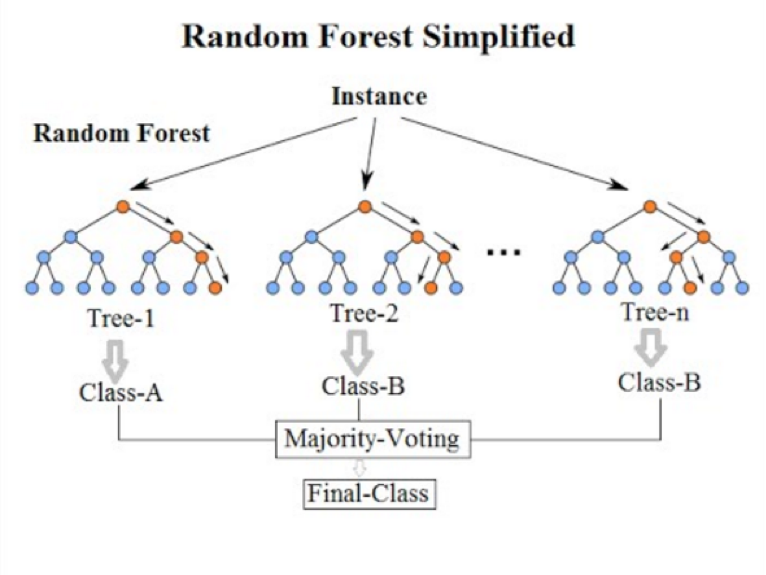
\includegraphics[width=9cm, height=8cm]{random_forest.png}\\
\caption{Random forest architecture}
\label{ran}
\end{figure}

Random Forest is one of the most popular machine learning algorithms for both classification and regression. The existing Prophet algorithm does not take advantage of the available past data, it only uses the current context information in its static model. Thus, it could be made more robust by integrating machine learning capabilities to it. Random forest uses the ensemble learning technique. By constructing several trees and taking an aggregate of them would only make the model robust as shown in Fig. \ref{ran}. Apart from this, it also provides better classification since it uses boosting and bagging techniques. It also helps in avoiding overfitting compared to their counterparts. Random forest is better suited for this particular application because it can work on multidimensional input data and the data used to train the model has a dimension greater than 50.
In an opportunistic network environment, each and every node contains the context and location information of its neighbors. This contextual information is used with the proposed model to make predictions. 
For a given node, extracted data about one neighbor at a time will be fed into trained model. Based on the features, the model classifies the neighbors as good forwarder or bad forwarder. After going through all the neighbors, data packets are forwarded to all of the good forwarders as explained in the Algorithm \ref{alg2}.  
Since it is an improvement over the Prophet algorithm, the Prophet probability is also considered one of the feature for classification. In order to see how the model performed in real world, the source code of the Prophet algorithm in one simulator was modified to include the trained model. 


\begin {algorithm}
\SetAlgoLined
\KwResult{Labelled dataset that can be fed into the model}
Begin \;
\ForEach{event $e$ in set $E$}{
	\ForEach{message $M$ in set $M_s$} {
	     \tcc {if key of the records are same and the current\_node and selected\_forwarder\_node are present successively in the path of the 
	     	message and message\_id in event e and message\_id in message M are same  }
     	\If{message\_id[M] == message\_id[e] and Key(e) == Key(M) and current\_node(e) + selected\_forwarder(e) in path[M]}{
     		delivery\_status[e] = "deliver"\;
     		processed[e] = True\;	
     }
    }
	\ForEach{event $e$ in set $E$ }{

		\If{processed[e] != True}{
			delivery\_status[e] = "not\_delivered"\;
			processed[e] = True
		}
	}
	\ForEach{event $e$ in set $E$}{
		remove processed[e]\;
	}
}
\caption{Labelling the dataset}
\label{alg1}
\end {algorithm}

%Algorithm \ref{alg1}, is used to create the final datasets from the intermediate datasets that were obtained from the simulation. The final dataset is used to train the random forest classifier to identify the capable and uncapable nodes. Line 2 loops through every event e in the event dataset. Line 3 loops through every message  M in the message information dataset Ms. Line 4-6 marks  a particular event e as \emph{delivered} if an event e resulted in the delivery of the message to the intended destination.  If a message M contains the \emph{current\_node} and \emph{selectedForwarder} of the event e in the path of M together, then the event e resulted in the delivery of the message and is marked as \emph{delivered} and \emph{Processed[e]} is set to True. Lines 9-14 marks the events with the Processed[e] = False as \emph{not delivered}.  This completes the labelling of the event datasets to the form suitable to be used for training the random forest classifier. Lines 15-16 deallocates the \emph{Processed} data.

\begin {algorithm}
\SetAlgoLined
Begin\;
\tcp{Original Prophet}
\ForEach{node $N_i$ as i}{
	dp[i] <-- $random()$
}
\For{every 5 seconds}{
	\ForEach{node $N_i$ as i}{
			dp[i] <-- $GetProphetProbabilty(i)$\;	
}
} 
\tcp{End of original Prophet}
\ForEach{message $m$ in current node $n$ buffer}{
	\ForEach{node $N_i$ as n in neighborhood set $G$}{
		    P(n) <-- dp[n]\;
		    \If{dp[n] $\geq$ $\l P(N_i)$}{
		    	\If{$N_i == X$}{
					update X\;
					update G\;					
				    Label = $RandomForest1(X, G, P(X), P(n))$\;
		    	}
				 \eIf{Label == "deliver"}{
					Relay the message to node $X$\;	 
			 }{\If{Label == "don\textquotesingle t deliver"}{
				Don't relay the message to the node $X$\;
	 		}}
	    } 
	    \If{dp[n] < $\l P(N_i)$}{
		    	\If{$N_i == X$}{
					update X\;
					update G\;					
				    Label = $RandomForest2(X, G, P(X), P(n))$\;
		    	}
				 \eIf{Label == "deliver"}{
					Relay the message to node $X$\;	 
			 }{\If{Label == "don\textquotesingle t deliver"}{
				Don't relay the message to the node $X$\;
	 		}}
	    } 
}
}
\caption{Improved Prophet algorithm}
\label{alg2}
\end {algorithm}
\section{Experimental Evaluation}

\subsection{Simulation Settings}
In this section, the performance of the proposed iProphet is evaluated using the Opportunistic Network Environment (ONE) \cite{keranen2008opportunistic} simulator. The simulation is done on a terrain size of  \(4,500 X 3,400 \) sq. m with 51 to 198 nodes deployed randomly. The transmission range of the node is set to 20 meters. The various parameters considered during simulation are shown in TABLE \ref{issues}. Here the proposed iProphet performance has been compared with Epidemic \cite{2000epi}, Prophet \cite{2003pric} and Spray and Wait  \cite{spyropoulos2005spray} routing protocols, under varying TTL values from 100 to 300 seconds, number of nodes from 51 to 198, and message creation interval from 25 to 35 seconds.
% The results are shown in Figs. \ref{one} to \ref{twelve}.

\begin{table*}
\footnotesize
 \centering
 %\tiny
  \begin{tabular}{|p{6cm}|p{6cm}|}
    \hline
    \textbf {Parameter} & \textbf {Value}  \\
     \hline
Simulation Area                             & (4,500 x 3,400) square meters          \\ \hline
Total number of nodes                       & 51-198                                    \\ \hline
Total group of nodes                        & 6                                      \\ \hline
Number of groups of pedestrains             & 3                                      \\ \hline
Number of nodes in each group of pedestrian & 30                                     \\ \hline
Walking speed of pedestrain                 & 0.5-1.5 km/h                           \\ \hline
Buffer size of pedestrain                   & 15 Mb                                  \\ \hline
Number of groups of tram                    & 3                                      \\ \hline
Number of nodes in each group of tram       & 2                                      \\ \hline
Speed of tran                               & 6.5 Km/h                               \\ \hline
Buffer size of tram                         & 59 Mb                                  \\ \hline
Bluetooth transmission speed                & 250 K                                  \\ \hline
Bluetooth transmission range                & 20 meters                              \\ \hline
High speed interface transmission speed     & 10 Mb                                  \\ \hline
High speed interface transmission range     & 1500 meters                            \\ \hline
Message time-to-live for each group         & 100  minutes                           \\ \hline
Message generation intervals                & 25-35 seconds                          \\ \hline
Message size                                & 500 Kb - 1 Mb                          \\ \hline
Node movement model                         & Shortage path map based movement model \\ \hline
Simulation time                             & 100000 seconds                         \\ \hline

  \end{tabular}
 \caption{Simulation Parameters}
  \label{issues}
\end{table*}
%\end{adjustbox}


\subsection{Simulation results and performance analysis}
In this section, Experimental evaluation of the iPRoPHET algorithm is provided by comparing it against Epidemic, PRoPHET, and SprayAndWait algorithms chosen as benchmarks, in terms of delivery probability, hop count, overhead ratio, average buffer time (in seconds), and average latency (in seconds), chosen as performance metrics, under varying number of Time-to-Live (TTL), number of nodes, and message generation interval respectively. Time-to-Live, number of nodes, message generation interval was varied between 100-300 seconds, 51-198 nodes, 25-35 to 65-75 secs respectively.


\begin{figure}[H]
\centering
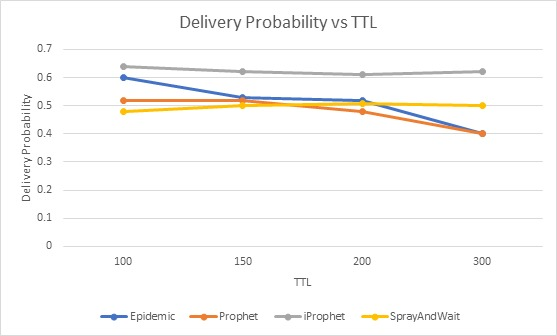
\includegraphics[width=9cm, height=8cm]{del_prob_vs_ttl.png}\\
\caption{Comparison of the delivery probability vs TTL.}
\label{one}
\end{figure}

\begin{figure}[H]
	\centering
	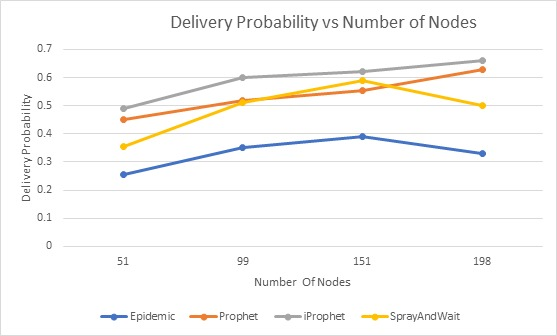
\includegraphics[width=9cm, height=8cm]{del_prob_vs_num_of_nodes.png}\\
	\caption{Comparison of the delivery probability vs number of nodes.}
	\label{four}
\end{figure}

\begin{figure}[H]
	\centering
	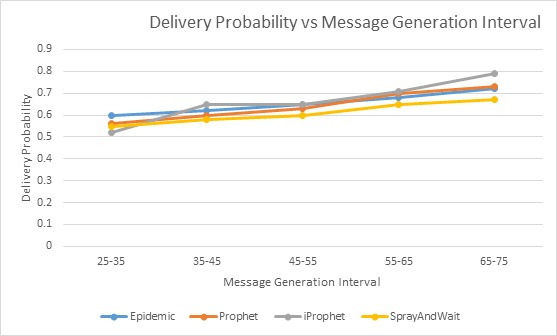
\includegraphics[width=9cm, height=8cm]{del_prob_vs_msg_gen_inter.png}\\
	\caption{Comparison of the delivery probablity vs message generation interval.}
	\label{eight}
\end{figure}


Fig \ref{one}, fig \ref{four} and fig \ref{eight} compares the delivery probability of various algorithms when the TTL, Number of Nodes and Message Generation Interval is varied in the manner described above. It can be observed that delivery probability of algorithms other than Epidemic and iPRoPHET decreases with the increase in TTL. This is due to the fact the lifetime of messages increases with the increase in TTL and hence the messages remain in the node buffer for longer time than usual which results in more messages getting dropped. However, in iPRoPHET algorithm, the delivery probability increases because of the selection of the next forwarder using random forest classifier which considers PRoPHET probability and other contextual information of the forwarders. The next forwarders are selected not only when their PRoPHET probability is greater but also when the probability is lower which helps to clear the messages from the buffer as quickly as possible. 
When the number of nodes is increased, the algorithm gets to work with more forwarders enhancing the delivery accuracy of the messages.
It can be observed that the iPRoPHET algorithm outperforms all other algorithms when it comes to delivery probability as the message generation interval is increased. When message interval is increased, the overhead of messages in the network reduces  and the router queues are free to accommodate the messages which reduces message dropping from the nodes buffer queue. This decrease in overhead ratio is depicted in fig 8.x(Overhead ratio vs Message Generation Interval). This, accompanied with the fit forwarders helps messages to get delivered to their respective destinations with improved probability.

\begin{figure}[H]
\centering
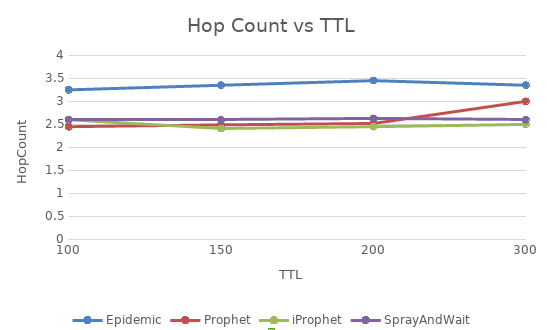
\includegraphics[width=9cm, height=8cm]{hop_count_vs_ttl.png}\\
\caption{Comparison of the hop count vs TTL.}
\label{two}
\end{figure}

\begin{figure}[H]
	\centering
	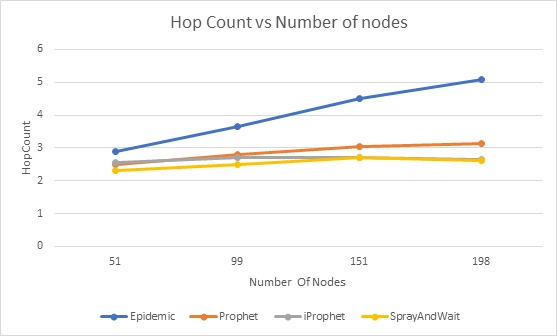
\includegraphics[width=9cm, height=8cm]{hop_count_vs_num_of_nodes.png}\\
	\caption{Comparison of the hop count vs number of nodes.}
	\label{five}
\end{figure}

\begin{figure}[H]
	\centering
	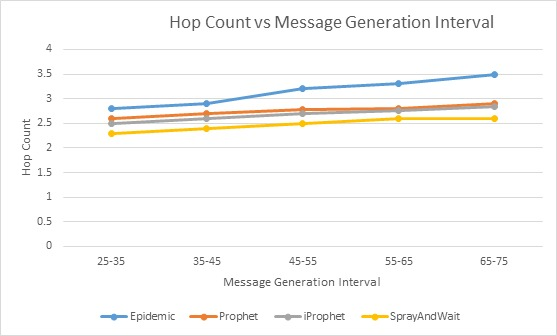
\includegraphics[width=9cm, height=8cm]{hop_count_vs_msg_gen_interval.png}\\
	\caption{Comparison of the hop count vs message generation interval.}
	\label{nine}
\end{figure}

Fig \ref{two}, fig \ref{five} and fig \ref{nine} compares the Hop Count of various algorithms when the TTL, Number of Nodes and Message Generation Interval is varied in the manner described above.
It can be seen that across all variations of TTL, number of nodes and message generation interval, iPRoPHET has a lesser hop count than PRoPHET algorithm. This is attributed to the fact that the iPRoPHET algorithm tries to maximize the delivery probability by even considering forwarders with lesser PRoPHET probability which could possibly have other better contextual attributes. When the number of nodes is increased, it leads to corresponding increase in number of forwarders available for routing the messages. Among these forwarders, the random forest classifier picks the fit nodes accurately leading to lesser overall hop count. Similar explanation holds when varied against TTL also. When TTL increases, hop count of other algorithms except SprayAndWait increases because of their nature of selection of forwarder nodes which are less likely to forward it to destination. Also, the messages stay in the buffer for longer period of time in PRoPHET since nodes won’t forward the messages if the PRoPHET probability is lower for the forwarders. When the message generation interval is varied, the number of messages in the network decreases, but the precision of the classifier remains same. Therefore, the overall decrease in hop count is observed across all the graphs. 

\begin{figure}[H]
\centering
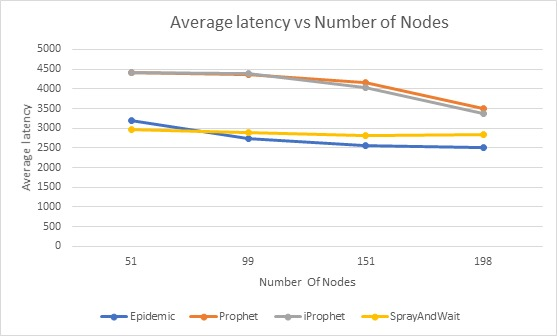
\includegraphics[width=9cm, height=8cm]{avg_lat_vs_num_of_nodes.png}\\
\caption{Comparison of the average latency vs number of nodes.}
\label{seven}
\end{figure}

\begin{figure}[H]
	\centering
	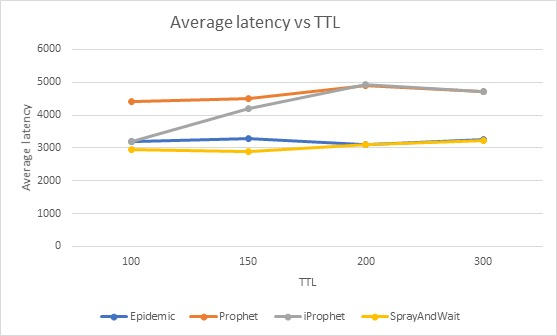
\includegraphics[width=9cm, height=8cm]{avg_lat_vs_ttl_n.png}\\
	\caption{Comparison of the average latency vs TTL.}
	\label{eleven}
\end{figure}

\begin{figure}[H]
	\centering
	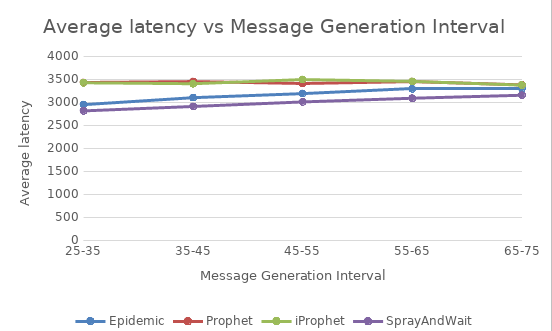
\includegraphics[width=9cm, height=8cm]{avg_lat_vs_msg_gen_inter_n.png}\\
	\caption{Comparison of the Average latency vs message generation interval.}
	\label{twelve}
\end{figure}

Fig \ref{seven}, fig \ref{eleven} and fig \ref{twelve} compares the average latency of various algorithms when the TTL, Number of Nodes and Message Generation Interval is varied in the manner described above.

iPRoPHET algorithm has only slightly lesser average latency time than PRoPHET because of the selection of the nodes with lesser PRoPHET delivery probability which is required to maximize the overall delivery probability but in doing that, the algorithm may select few outliers that might keep the messages for far longer time than usual and as number of nodes, the outlier count increases which increases the message delivery latency. However, this is compensated by the lesser hop count delivery of the non-outlier nodes that help to keep the latency times in control for majority of the messages. Similar impact of outliers can be seen when the TTL and message generation interval is varied. But the majority of non-outlier nodes overcome such impact with their timely delivery of the messages to their destinations.



Fig. \ref{nine} compares the Hop Count of various algorithms when the message generation interval is varied from 25-35 to 65-75. When Prophet and iProphet are compared, the hop count is slightly lesser for iProphet algorithm. This is attributed to the fact that the iProphet algorithm tries to maximize the delivery probability by even considering forwarders with lesser Prophet probability which could possibly have other better contextual attributes. As a result, messages move through lesser number of hops than Prophet.


\begin{figure}[H]
\centering
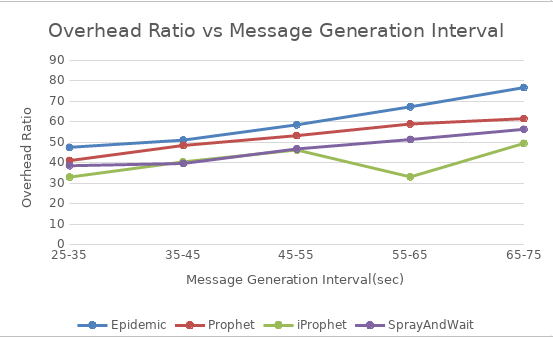
\includegraphics[width=9cm, height=8cm]{oh_ratio_vs_msg_gen_inter.png}\\
\caption{Comparison of the overhead ratio vs message generation interval.}
\label{ten}
\end{figure}

Fig. \ref{ten} compares the overhead ratio of various algorithms
when the message generation interval is varied from 25-35
to 65-75. It is observed that the overhead ratio is better in
iProphet because of the increased delivery probability result-
ing from better forwarders chosen as part of random forest
classifier.

\begin{figure}[H]
	\centering
	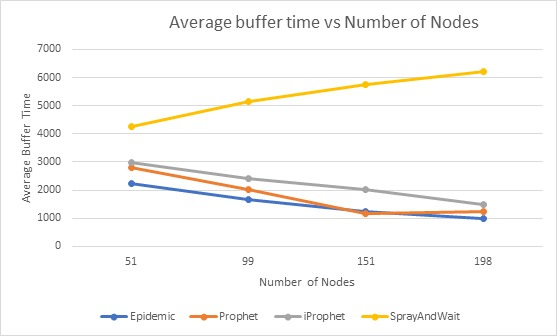
\includegraphics[width=9cm, height=8cm]{avg_buff_time_vs_num_of_nodes.png}\\
	\caption{Comparison of the average buffer time vs number of nodes.}
	\label{six}
\end{figure}

\begin{figure}[H]
	\centering
	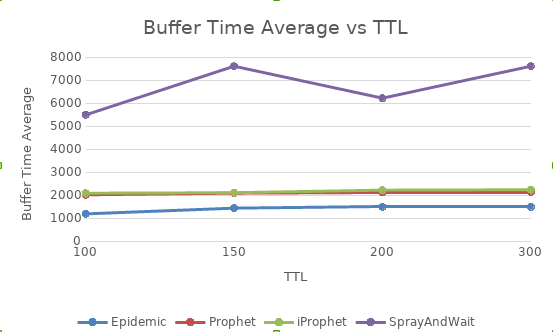
\includegraphics[width=9cm, height=8cm]{buf_time_vs_ttl.png}\\
	\caption{Comparison of the buffer time average vs ttl.}
	\label{three}
\end{figure}

Fig \ref{six} and Fig \ref{three} compares the average buffer time of various algorithms when the number of nodes and TTL is varied in the manner described above.. iPRoPHET algorithm has slightly greater average buffer time because of the selection of the nodes with lesser PRoPHET delivery probability which is required to maximize the overall delivery probability but in doing that, the algorithm may select few outliers that might keep the messages for far longer time than usual and as number of nodes increases, the outlier count increases keeping the average buffer time slightly larger and outlier prone. 
When the TTL is increased, the similar impact of outliers can be seen. The messages stay in the outlier nodes buffer for longer time than usual without getting forwarded and therefore add to the increased average buffer time.



\section{Conclusions and future work}
In this paper multi-copy routing algorithm for opportunistic networks named iProphet or improved Prophet is proposed. This method makes use of machine learning classifier called random forest and delivery probability of existing Prophet to establish routing of messages. With the simulation results it can be concluded that: (i) While making each routing decision, random forest classified the nodes as reliable or unreliable which led to better selection of intermediate nodes for carrying out the routing task leading to efficient routing. (ii) Proposed method outperforms in terms of delivery probability, hop count, overhead ratio and latency in comparison with similar existing algorithms. (iii) The classifier trained with large amount of data extracted using simulation leads to precise classification of the nodes as reliable or unreliable for carrying out the routing task. However the proposed method will have poor performance in terms of average buffer time in par with similar multi-copy routing algorithm. \\
The average buffer time has experienced a performance issue due to the presence of the outlier nodes, which needs to be addressed as part of future enhancement. Furthermore, energy consumption of the nodes needs to be optimized for working with compute-intensive machine learning algorithms. 

\section{Acknowledgment}
This research work has been funded by the Science and Engineering Research Board (SERB-DST) Project File No: EEQ/2017/000681. Authors sincerely thank SERB-DST for intellectual generosity and research support provided.


\bibliography{MAGSA}
\bibliographystyle{unsrt}
\end{document}
